\documentclass{article}
\usepackage{../fasy-hw}

%% UPDATE these variables:
\renewcommand{\hwnum}{3}
\title{Discrete Structures, Homework \hwnum}
\author{Patrick O'Connor (Patrick OConnor (322))}
\collab{n/a}
\date{due: 19 February 2021}

\begin{document}

\maketitle

This homework assignment should be
submitted as a single PDF file both to D2L and to Gradescope.

General homework expectations:
\begin{itemize}
    \item Homework should be typeset using LaTex.
    \item Answers should be in complete sentences and proofread.
    \item You will not plagiarize.  \item List collaborators at the start of
    each question using the \texttt{collab} command.
    \item Put your answers where the \texttt{todo} command currently is (and
        remove the \texttt{todo}, but not the word \texttt{Answer}).
\end{itemize}

% ============================================
% ============================================
\collab{n/a} \nextprob{Negations}
% ============================================
% ============================================
Negate the following statements:

\begin{enumerate}

    \item Each ``Clean 'Cat Kit''  contains a cloth mask and a refillable hand
        sanitizer.

        \paragraph{Answer}
        There exists a `Clean 'Cat Kit'' that does not contain a cloth mask
        and a refillable hand
        sanitizer.

    \item There exists a boat docked in New Jersey that I have steered.

        \paragraph{Answer}
        I have not steered any of the boats docked in New Jersey.

    \item There exists an island in the Ohio River with a bowling alley and a
        university track field.

        \paragraph{Answer}
        On the Ohio River there is not an island with a bowling alley and
        university track field.

    \item Both my sister and I can climb every route at Spire.

        \paragraph{Answer}
        There exists a route at Spire that my sister and I can not climb

\end{enumerate}

% ============================================
% ============================================
\collab{n/a} \nextprob{Definitions}
% ============================================
% ============================================
Use the definitions provided in the course textbook to prove that every prime
number except~$2$ is odd.

\paragraph{Answer}

  Lemma:  $\forall n \in \Z$, n is even if $n=2k$.
  Let $P \in \Z$. \\
  $\forall$ r, s $\in \Z$,
  if $P = rs$, then ($r=1 \land s=P$)$\lor$($s=1 \land r=P$) \\
  Let P $\in \Z$ \\
  By definition of a prime number,
  $\forall$ P, $P/P=1$ or $P/1=P$ and P is not prime if $P$/(P or 1)$ \neq$
  (1 or P respectively). By the above Lemma all even numbers are divisible
  by 2.\\
  Therefore, all prime numbers > $2$ are odd.


%
% ============================================
% ============================================
\collab{n/a}
\nextprob{Four Colors Suffice}
% ============================================
% ============================================
Read Chapters $2$ and $3$ of \emph{Four Colors Suffice} and answer the following
 questions:

\begin{enumerate}

    \item Who are the Austrian(s) mentioned in Chapters $1$--$3$, and what was
    their contribution mentioned in the book?

        \paragraph{Answer}
        The Austrian mentioned in Chapter $2$ is Heinrich Tietze. Teitze
        described a situation in which more than four colors are necessary in
        for three-dimensional maps. This situation involves taking a number of
        horizontal bars numbers $1$ to $n$, that have vertical bars also
        numbered $1$ to $n$. These are joined as a single country  if horizontal
        and vertical numbers match.
        This is similar to jenga blocks in a pile or legos blocks.
        After joining into countries, we have n three dimensional countries
         that are all touching each other.
        Therefore we would need n colors which if n is greater than ,
        the four color theorem does not apply.

    \item Write a statement of the four color theorem using a universal
        quantifier.

        \paragraph{Answer}
        For all maps $m$, there are at-least four colors needed to color it such
        that no same color comes into contact at more than a point.

    \item What is the definition of a $k$-coloring of a graph?

        \paragraph{Answer}
        A graph $G  = (V,E)$ is of a $k$-coloring if each vertex can be assigned
         a color in ${1,...,k}$ so that no edge has two vertices of the same
         coloring.

    \item Prove or disprove: all plane graphs are three-colorable.

        \paragraph{Answer}
        By definition a plane graph is a graph that can be drawn on a 2d
        surface or plane. The edges of the graph may only intersect at the
        vertices. The figure below follows the guidelines and is not
        three-colorable. Therefore, there exists a plane graph that is not
        three-colorable and the statement all plane graphs are three-
        colorable is false.
        \begin{figure}
          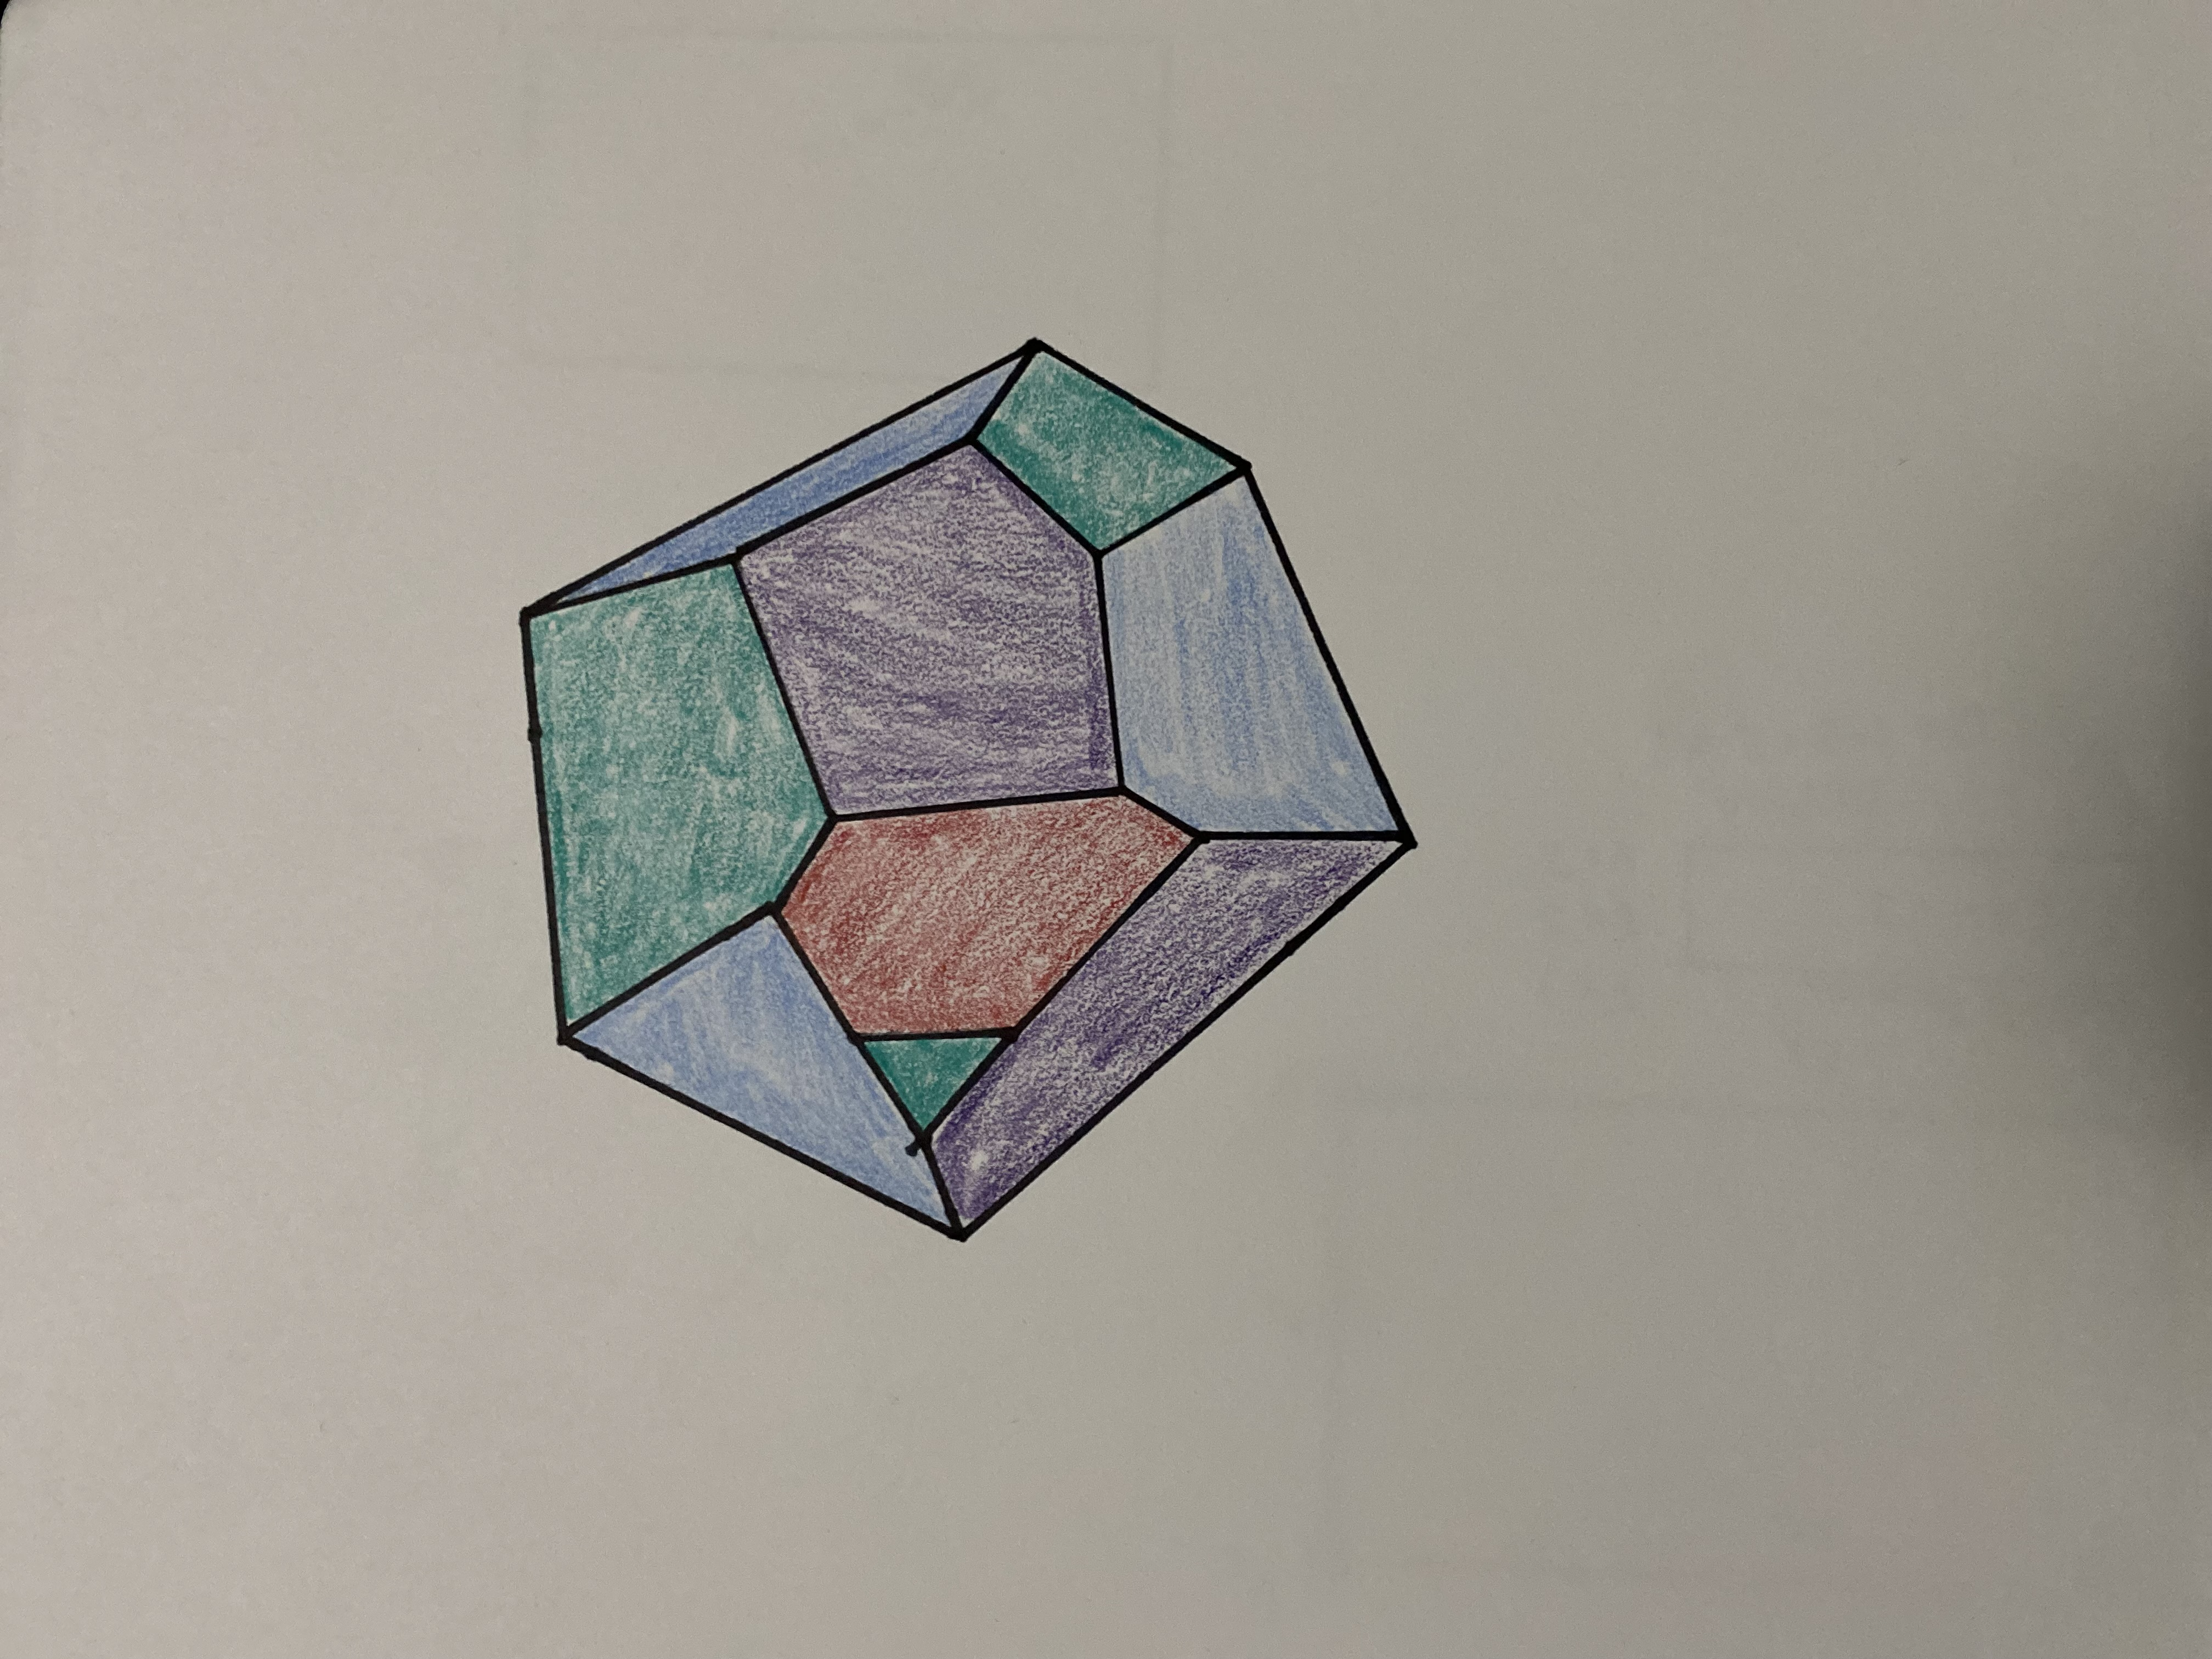
\includegraphics[width=\linewidth]{4-color-graph.png}
          \caption{A plane graph that is at least 4 colorable}
          \label{fig:4-color-graph}
        \end{figure}
Figure \ref{fig:chessboard} A two-coloring map example: Chessboard.

    \item Assuming the four color theorem holds, prove or disprove: six colors
        suffice to color a plane graph.

        \paragraph{Answer}
        Lemma 1. For any simple planar graph G, the average degree of G is
        strictly less than 6.

        Assume any simple planar graph can be properly colored with six colors.

        For any connected plane graph $G$, the faces or vertices can be
        colored in 6 or fewer colors with no touching similar colors. Using the
        definition for $k$-coloring of graphs there is a function that exists
        where $V(G) = {1,2,3,...,k}$ where $1 \geq \ k \leq \ 6$ such that
        for every x, y $\in$ V(G), $f(x) \neq f(y)$.

        Let $G$ be any planar graph on $v = n+1$ where $v$ is vertices. From
        the lemma above we know that $G$ must have some vertex $z$ where the
        degree is $w \leq 5$. By removing $w$ from the graph we can form
        $G\prime$. $G\prime$ has $v = n$ vertices and through induction we can
        know that $G\prime$ can be colored in 6 colors. With all but $z$ colored
        and because we know that at most w has a degree of 5, we can color $z$
        with one of the colors that is not neighboring.



    \item Give an example of a map with at least five faces that has a
        two-coloring.  Be sure to provide a coloring as evidence that the map is
        two-colorable.

        \paragraph{Answer}
        An example of a map that has atleast 5 faces and is two-coloring is
        a chess or checkboard. The figure below is a colored in chessboard
        that has 64 faces and only a two colors are used in accordance with
        coloring standards.
        \begin{figure}
          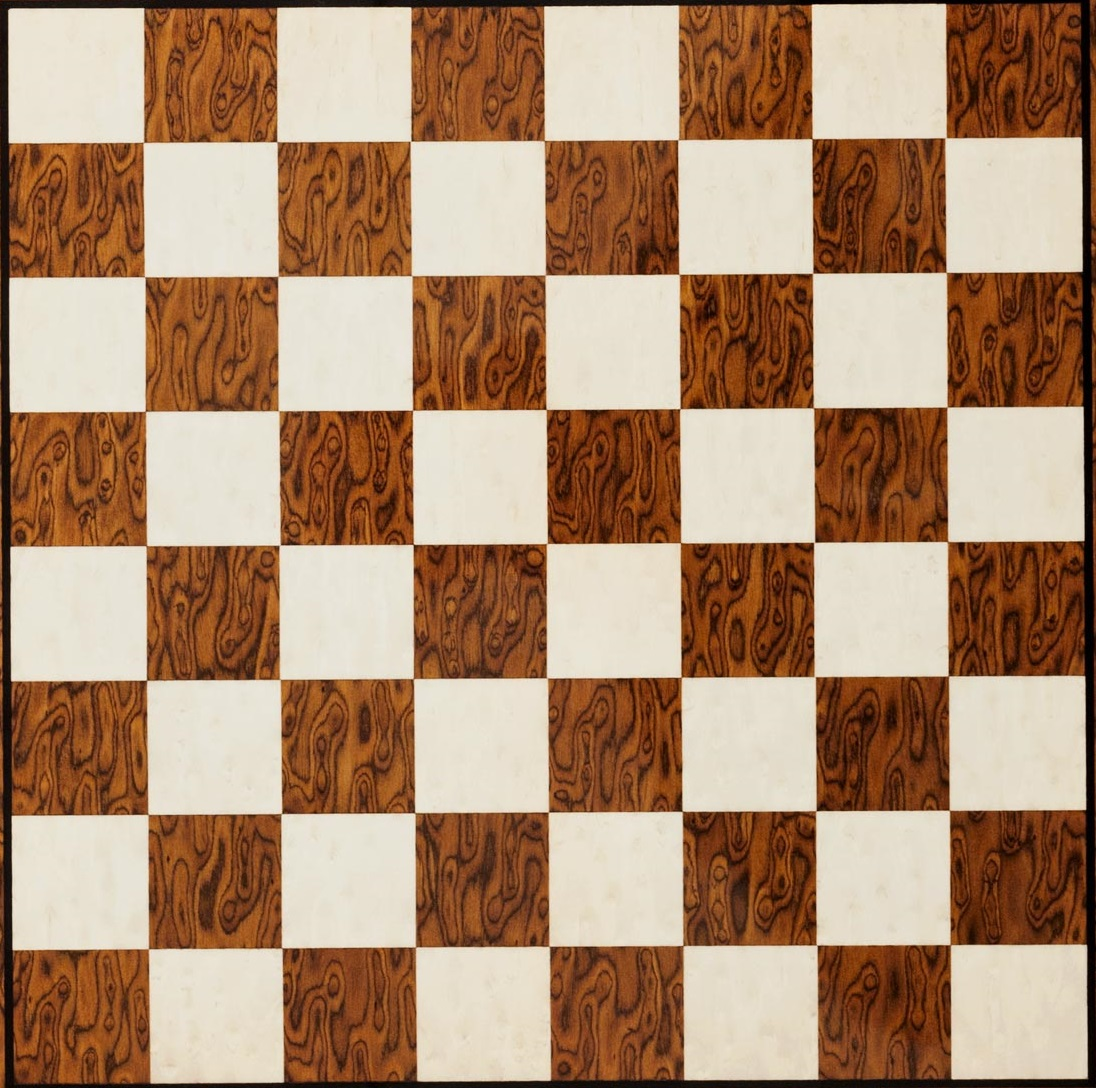
\includegraphics[width=\linewidth]{chess.png}
          \caption{A two-coloring example: Chessboard.}
          \label{fig:chessboard}
        \end{figure}
Figure \ref{fig:chessboard} A two-coloring map example: Chessboard.

    \item Euler's formula states that if we have a map on the sphere or plane
        and count the exterior face as a face, then F-E+V=2.  Does this equation
        hold if the map is drawn on a M\"obius band? Why or why not? (Note:
        here, the boundary of the M\"obius band must be represented in the graph
        defining the map, and no ``country'' can be on the same side of a single
        edge.)

        \paragraph{Answer}
        This formula does not hold true for some maps drawn on a M\"obius band.
        An example of a map that does not follow Euler's formula of F-E+V=2 as
        the values are $F=1$, $E=3$, $V=2$. When this is plugged into the
        formula the result is $1-3+2 \neq 2 = 0$. Therefore at least some of the
        maps drawn on a M\"obius band do not fit Euler's formula.
        \begin{figure}
          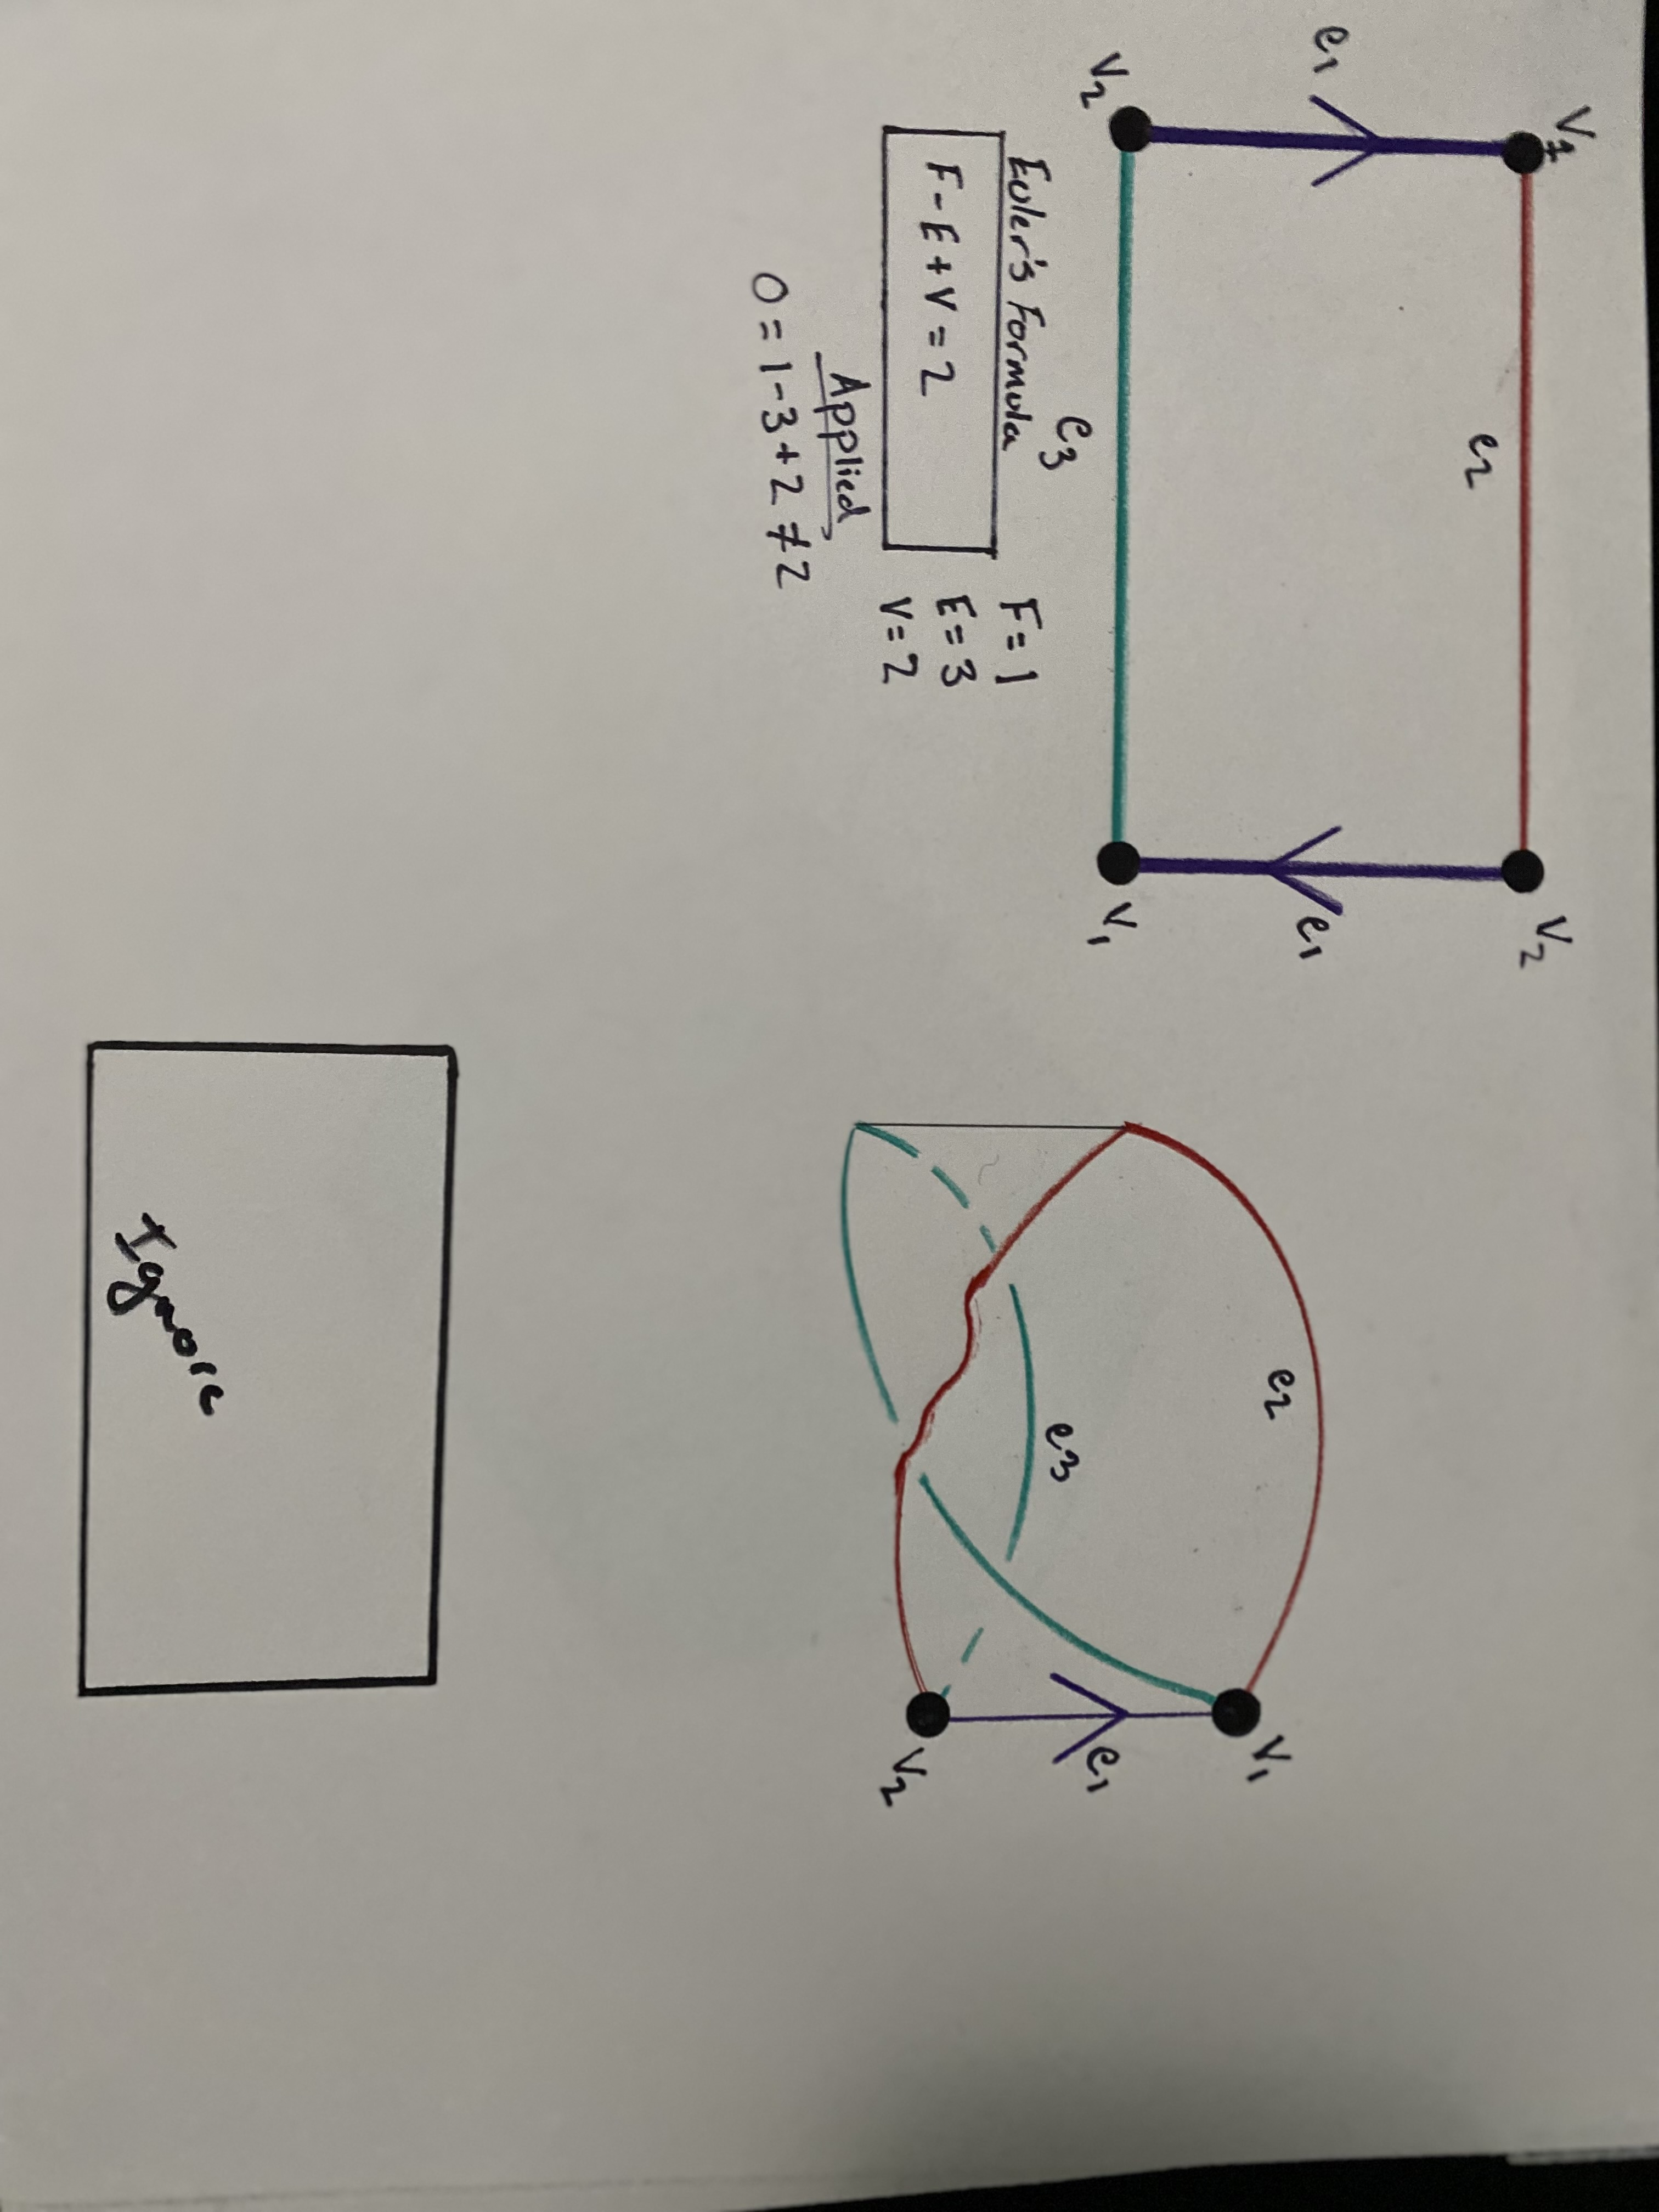
\includegraphics[width=\linewidth]{mobius.png}
          \caption{A M\"obius band that breaks Euler's formula}
          \label{fig:mobius}
        \end{figure}
        Figure \ref{fig:mobius} A M\"obius band that breaks Euler's formula

    \item In your own words, explain the joke: ``A topologist cannot tell the
        difference between a coffee cup and a donut.''  You are encouraged to
        use Wikipedia to formulate your answer, but be sure to cite sources.

        \paragraph{Answer}
        A topologist cannot tell the difference between a coffee cup and a
        donut is a joke made based on the that in mathematics topology is
        only concerned with the properties of an object that are under
        continous deformations(Wikipedia). The basis on which a coffe mug
        is a donut in a topologist mind is that through stretching, twisting,
        and crumpling it is possible to deform a mug into a donut or back to the
        other shape. In mathematic topology tearing and glueing are not allowed
        which is essential for understanding the joke. The most important
        similarity is that each have a hole(donut = center hole, mug =
        handle whole). Starting at the mug we can stretch up the base to
        un-cup it then smash and stretch the cup portion into the handle.
        From there we have a misshaped donut and with a bit more distortion we
        can smooth the uneven donut into a perfectly round donut.

\end{enumerate}

% ============================================
% ============================================
\collab{n/a}
\nextprob{Ada Lovelace}
% ============================================
% ============================================

Write a short (1-2 paragraph) biography of Ada Lovelace.
\textbf{In your own words}, describe who they are and why they are important in
the history of computer science.  If you use external resources, please provide
proper citations (see the `hw/bib-ex` folder for examples of how to use
citations). If you do not use external sources, please write ``I did not
use any sources to write this biography'' as the last sentence of the
\paragraph{Answer}

Ada Lovelace was an English mathematician during the early 1800's.
Ada Lovelace was a highly educated human who came from fame and fortune.
Her father was a famed poet Lord Byron, who is known for his romantic and
satirist poetry that represented Europe's imagination. Although this fame
most likely assisted in affording the private tutoring, Lord Byron left Britain
before Ana ever met him. She was privately educated by Augustus De Morgan who
you may know from De Morgan's laws which states that mathematical statements
and concepts are related through their oppositions/opposites.
After marrying into royalty in the 1830's, she pursued understanding and
progressing the pursuit of early computing that had been started
by Charles Babbage.

Within her work on Charles Babbage's proposed computer, the Analytical Engine,
she explored the ability for the Analytical Engine to follow a series of steps.
These steps would in today's language would be considered a program.
Her discovery of the ability for the Analytical Engine to follow steps was
found when translating and annotating an article written by Luigi Federico
Menabrea. Her deep understanding of the Analytical Engine assisted in writing
detailed annotations on how the computing device could calculate Bernoulli
numbers. At this point the detailed annotations were not system instructions
but rather an algorithm that stepped through instructions.
Along with defining what some would say is the first program,
she devised a vision for computers to be used as tools to interact
with other types of data such as words.

% %% ... the bibliography
% \newpage
% \bibliographystyle{acm}
% \bibliography{biblio}

\end{document}
